\documentclass{report}

\usepackage[english]{babel}
\usepackage[letterpaper,top=2cm,bottom=2cm,left=3cm,right=3cm,marginparwidth=1.75cm]{geometry}
\usepackage{amsmath}
\usepackage{amsfonts} 
\usepackage{graphicx}
\usepackage[colorlinks=true, allcolors=blue]{hyperref}
\graphicspath{{images/}}
\setcounter{tocdepth}{4}
\setcounter{secnumdepth}{4}
\usepackage[table,xcdraw]{xcolor}
\usepackage{float}
\usepackage{listings}
% More defined colors
 
% Required package
\usepackage{tikz}
 

\title{Properties of relations on a set determined by a matrix}

\author{Mr Ashlin Darius Govindasamy\\ \large{University of South Africa} \\ \large{Department of Computer Science and Mathematics}}
\date{\today}


\begin{document}
\maketitle
\newpage


\begin{abstract}
This paper introduces a technique of converting a relation set into a matrix of $\mathbb{R}^{n}$ space using that matrix classifying the properties for the relational set.
Using this technique, we can find the properties of a relation set by using some properties of the matrix. In programming, we can use this technique to determine our properties of a relation set by using the matrix. Code snippets are provided to show how this technique can be used in programming.
\end{abstract}

\newpage
\tableofcontents

%for adding page numbers
\pagenumbering{arabic} 


%add more chapters like this
\chapter{Relations}
%add subsections like this
\subsection{What is a relation?}

A (binary) relation $R$ between sets $A$ and $B$ is a subset of $A \times B$. ($A \times B$ is a Cartesian product.) 

Thus, a relation is a set of pairs. 

The interpretation of this subset is that it contains all the pairs for which the relation is true.  We write $aRb$ if the relation is true for $A$ and $B$ (equivalently $B$, if $(A,B) \in R$). 

$A$ and $B$ can be the same set, in which case the relation is said to be "on" rather than "between":

A binary relation $R$ on a set $A$ is a $\subseteq$ $A \times A$. ($A \times A$ is a Cartesian product.) \\

Example of a relation using $A = \{0,1,2,3\}$ \\

 \begin{math}
    R = \{(0,0),(1,1),(2,2),(3,3)\}  \\
\end{math}

Relations may also be of other arities.  An $n$-ary relation $R$ between sets $X_{1}$, ... , and $X_{n}$ $\subseteq$  $n$-ary product $X_{1}$...$X_{n}$, in which case R is a set of n-tuples. 

\subsubsection{Some specific relations}
The empty relation between sets X and Y, or on E, is the empty set $\emptyset$. 

The empty relation is false for all pairs. 

The full relation (or universal relation) between sets X and Y is the set X$\times$Y. 

The full relation on set E is the set E$\times$E. 

The full relation is true for all pairs. 

The identity relation on set E is the set ${(x,x) | x\in{E}}$. 

The identity relation is true for all pairs whose first and second element are identical. 



\subsection{Properties of relations}

\begin{table}[H]
    \centering
    \resizebox{\textwidth}{!}{%
    \begin{tabular}{|l|l|}
    \hline
    \multicolumn{1}{|c|}{\textbf{A relation R is..}} & \multicolumn{1}{c|}{\textbf{if ...}}            \\ \hline
    \textit{\textbf{reflexive}}                      & xRx                                             \\ \hline
    \textit{\textbf{symmetric}}                      & xRy implies yRx                                 \\ \hline
    \textit{\textbf{transitive}}                     & \cellcolor[HTML]{FFFFFF}xRy and yRz implies xRz \\ \hline
    \textit{\textbf{irreflexive}}                    & \cellcolor[HTML]{FFFFFF}xRy implies x$\neq$y         \\ \hline
    \textit{\textbf{antisymmetric}}                  & xRy and yRx implies x=y                         \\ \hline
    \textit{\textbf{triohotomy}}                     & xRy or x=y or yRx                               \\ \hline
    \end{tabular}%
    }
\end{table}

\subsubsection{Reflexive}
Let Relation $R$ on $A$ \\
Where $R \subseteq A \times A$

The reflexive property of a relation is that $\forall a \in A$, $aRa$ is true.

Also could be written as $R \subseteq A \times A$ and $\forall a \in A$, then $(a,a) \in R$

\textbf{Example:}

Let $A = \{1,2,3,4\}$ \\
Let $R = \{(1,1),(2,2),(2,3),(3,4),(3,3),(4,4),(4,2)\}$ \\

We could draw a matrix to show the relation $R$ on $A$ \\

To draw the matrix we plot the elements of $A$ on the x-axis and y-axis. \\
Then we plot the pairs of $R$ on the matrix as 1. \\
If the pair is not in $R$ then we plot a 0. \\

 
\begin{tabular}{|c|c|c|c|c|}
\hline
\multicolumn{1}{|c|}{\textbf{}} & \multicolumn{1}{c|}{\textbf{1}} & \multicolumn{1}{c|}{\textbf{2}} & \multicolumn{1}{c|}{\textbf{3}} & \multicolumn{1}{c|}{\textbf{4}} \\ \hline
\multicolumn{1}{|c|}{\textbf{1}} & \multicolumn{1}{c|}{\textbf{1}} & \multicolumn{1}{c|}{\textbf{0}} & \multicolumn{1}{c|}{\textbf{0}} & \multicolumn{1}{c|}{\textbf{0}} \\ \hline
\multicolumn{1}{|c|}{\textbf{2}} & \multicolumn{1}{c|}{\textbf{0}} & \multicolumn{1}{c|}{\textbf{1}} & \multicolumn{1}{c|}{\textbf{1}} & \multicolumn{1}{c|}{\textbf{0}} \\ \hline
\multicolumn{1}{|c|}{\textbf{3}} & \multicolumn{1}{c|}{\textbf{0}} & \multicolumn{1}{c|}{\textbf{0}} & \multicolumn{1}{c|}{\textbf{1}} & \multicolumn{1}{c|}{\textbf{1}} \\ \hline
\multicolumn{1}{|c|}{\textbf{4}} & \multicolumn{1}{c|}{\textbf{0}} & \multicolumn{1}{c|}{\textbf{1}} & \multicolumn{1}{c|}{\textbf{0}} & \multicolumn{1}{c|}{\textbf{1}} \\ \hline
\end{tabular} \\

We can also draw a directional graph to show the relation $R$ on $A$ \\
We plot the elements of $A$ as nodes. \\
We plot the pairs of $R$ as directed edges. \\

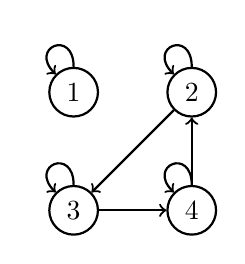
\begin{tikzpicture}[node distance={15mm}, thick, main/.style = {draw, circle}] 
    \node[main] (1) {$1$}; 
    \node[main, right of=1] (2) {$2$};
    \node[main, below of=1] (3) {$3$};
    \node[main, below of=2] (4) {$4$};
    \draw[->] (1) to [out=90,in=135,looseness=5] (1);
    \draw[->] (2) to [out=90,in=135,looseness=5] (2);
    \draw[->] (2) to (3);
    \draw[->] (3) to (4);
    \draw[->] (3) to [out=90,in=135,looseness=5] (3);
    \draw[->] (4) to [out=90,in=135,looseness=5] (4);
    \draw[->] (4) to (2);
\end{tikzpicture} \\


Thus resulting in the relation $R$ being reflexive. \\
This is because for all $a \in A$, $aRa$ is true. \\
For example, $1R1$ is true, $2R2$ is true, $3R3$ is true, $4R4$ is true. \\
Therefore $R$ is reflexive. \\

In the matrix, we can see that the diagonal is all 1's. \\
If you notice, the diagonal is the pairs $(a,a)$ for all $a \in A$. \\
In programming we look at this problem as a 2D array. \\

Using Mathematics logic, we can write this as: \\
$R \subseteq A \times A$ and $\forall a \in A$, then $(a,a) \in R$ \\

Where $R$ is a 2D array. \\

Or in psuedocode: \\

\begin{lstlisting}
function isReflexive(R)
    bValid = True
    for i = 0 to R.length
        for j = 0 to R.length
            if R[i][j] = 0 
                bValid = False
            end if
        end for
    end for                    
    return bValid
\end{lstlisting}

\subsubsection{Irreflexive}
Let Relation $R$ on $A$ \\
Where $R \subseteq A \times A$

The irreflexive property of a relation is that $\forall a \in A$, $aRa$ is false.

Also could be written as $R \subseteq A \times A$ and $\forall a \in A$, then $(a,a) \notin R$

\textbf{Example:}

Let $A = \{1,2,3,4\}$ \\
Let $R = \{(1,2),(2,3),(3,4),(4,1)\}$ \\
We could draw a matrix to show the relation $R$ on $A$ \\
To draw the matrix we plot the elements of $A$ on the x-axis and y-axis. \\
Then we plot the pairs of $R$ on the matrix as 1. \\
If the pair is not in $R$ then we plot a 0. \\


\begin{tabular}{|c|c|c|c|c|}
\hline
\multicolumn{1}{|c|}{\textbf{}} & \multicolumn{1}{c|}{\textbf{1}} & \multicolumn{1}{c|}{\textbf{2}} & \multicolumn{1}{c|}{\textbf{3}} & \multicolumn{1}{c|}{\textbf{4}} \\ \hline
\multicolumn{1}{|c|}{\textbf{1}} & \multicolumn{1}{c|}{\textbf{0}} & \multicolumn{1}{c|}{\textbf{1}} & \multicolumn{1}{c|}{\textbf{0}} & \multicolumn{1}{c|}{\textbf{0}} \\ \hline
\multicolumn{1}{|c|}{\textbf{2}} & \multicolumn{1}{c|}{\textbf{0}} & \multicolumn{1}{c|}{\textbf{0}} & \multicolumn{1}{c|}{\textbf{1}} & \multicolumn{1}{c|}{\textbf{0}} \\ \hline
\multicolumn{1}{|c|}{\textbf{3}} & \multicolumn{1}{c|}{\textbf{0}} & \multicolumn{1}{c|}{\textbf{0}} & \multicolumn{1}{c|}{\textbf{0}} & \multicolumn{1}{c|}{\textbf{1}} \\ \hline
\multicolumn{1}{|c|}{\textbf{4}} & \multicolumn{1}{c|}{\textbf{1}} & \multicolumn{1}{c|}{\textbf{0}} & \multicolumn{1}{c|}{\textbf{0}} & \multicolumn{1}{c|}{\textbf{0}} \\ \hline
\end{tabular} \\
We can also draw a directional graph to show the relation $R$ on $A$ \\
We plot the elements of $A$ as nodes. \\
We plot the pairs of $R$ as directed edges. \\
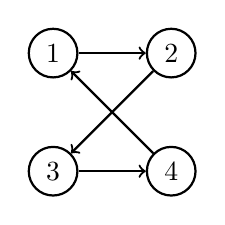
\begin{tikzpicture}[node distance={15mm}, thick, main/.style = {draw, circle}] 
    \node[main] (1) {$1$}; 
    \node[main, right of=1] (2) {$2$};
    \node[main, below of=1] (3) {$3$};
    \node[main, below of=2] (4) {$4$};
    \draw[->] (1) to (2);
    \draw[->] (2) to (3);
    \draw[->] (3) to (4);
    \draw[->] (4) to (1);
\end{tikzpicture} \\
Thus resulting in the relation $R$ being irreflexive. \\
This is because for all $a \in A$, $aRa$ is false. \\
For example, $1R1$ is false, $2R2$ is false, $3R3$ is false, $4R4$ is false. \\
Therefore $R$ is irreflexive. \\
In the matrix, we can see that the diagonal is all 0's. \\
If you notice, the diagonal is the pairs $(a,a)$ for all $a \in A$. \\
In programming we look at this problem as a 2D array. \\
Using Mathematics logic, we can write this as: \\
$R \subseteq A \times A$ and $\forall a \in A$, then $(a,a) \notin R$ \\
Where $R$ is a 2D array. \\
Or in psuedocode: \\
\begin{lstlisting}
function isIrreflexive(R)
    bValid = True
    for i = 0 to R.length
        for j = 0 to R.length
            if R[i][j] = 1 
                bValid = False
            end if
        end for
    end for                    
    return bValid
\end{lstlisting}

If you want to be real and save time coding.
\begin{lstlisting}
    function isIrreflexive(R)
        return isReflexive(R)
    end function
\end{lstlisting}

\subsubsection{Symmetric}
Let Relation $R$ on $A$ be symmetric if $\forall a,b \in A$ then $(a,b) \in R$  $(b,a) \in R$ \\

\textbf{Example:}
$R ={(1,1),(1,3),(2,3),(2,4),(3,1),(3,2),(4,2)}$ \\
We can draw a matrix to show the relation $R$ on $A$ \\
To draw the matrix we plot the elements of $A$ on the x-axis and y-axis. \\
Then we plot the pairs of $R$ on the matrix as 1. \\
If the pair is not in $R$ then we plot a 0. \\

\begin{tabular}{|c|c|c|c|c|}
\hline
\multicolumn{1}{|c|}{\textbf{}} & \multicolumn{1}{c|}{\textbf{1}} & \multicolumn{1}{c|}{\textbf{2}} & \multicolumn{1}{c|}{\textbf{3}} & \multicolumn{1}{c|}{\textbf{4}} \\ \hline
\multicolumn{1}{|c|}{\textbf{1}} & \multicolumn{1}{c|}{\textbf{1}} & \multicolumn{1}{c|}{\textbf{0}} & \multicolumn{1}{c|}{\textbf{1}} & \multicolumn{1}{c|}{\textbf{0}} \\ \hline
\multicolumn{1}{|c|}{\textbf{2}} & \multicolumn{1}{c|}{\textbf{0}} & \multicolumn{1}{c|}{\textbf{0}} & \multicolumn{1}{c|}{\textbf{1}} & \multicolumn{1}{c|}{\textbf{1}} \\ \hline
\multicolumn{1}{|c|}{\textbf{3}} & \multicolumn{1}{c|}{\textbf{1}} & \multicolumn{1}{c|}{\textbf{1}} & \multicolumn{1}{c|}{\textbf{0}} & \multicolumn{1}{c|}{\textbf{0}} \\ \hline
\multicolumn{1}{|c|}{\textbf{4}} & \multicolumn{1}{c|}{\textbf{0}} & \multicolumn{1}{c|}{\textbf{1}} & \multicolumn{1}{c|}{\textbf{0}} & \multicolumn{1}{c|}{\textbf{0}} \\ \hline
\end{tabular} \\

We can also draw a directional graph to show the relation $R$ on $A$ \\
We plot the elements of $A$ as nodes. \\
We plot the pairs of $R$ as directed edges. \\
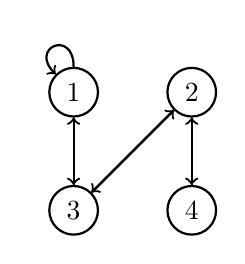
\begin{tikzpicture}[node distance={15mm}, thick, main/.style = {draw, circle}] 
    \node[main] (1) {$1$}; 
    \node[main, right of=1] (2) {$2$};
    \node[main, below of=1] (3) {$3$};
    \node[main, below of=2] (4) {$4$};
    \draw[->] (1) [out=90,in=135,looseness=5] to (1);
    \draw[->] (1) to (3);
    \draw[->] (2) to (3);
    \draw[->] (2) to (4);
    \draw[->] (3) to (1);
    \draw[->] (3) to (2);
    \draw[->] (4) to (2);     
\end{tikzpicture} \\

Notice that the relation $R$ is symmetric. \\
This is because for all $a,b \in A$, $aRb$ is true. \\
$aRb$ is true if and only if $bRa$ is true. \\
For example, $1R1$ is true, $1R3$ is true, $2R3$ is true, $2R4$ is true, $3R1$ is true, $3R2$ is true, $4R2$ is true. \\
Therefore $R$ is symmetric. \\
In the matrix, we can see that the matrix is symmetric. \\

Using our knowledge of matrices, we can write this as: \\
$R \subseteq A \times A$ and $R = R^T$ \\
Where $R$ is a 2D array. \\

Remember that $R^T$ is the transpose of $R$. \\
The transpose of a matrix is the matrix found by interchanging its rows into columns or columns into rows.\\
In programming we look at this problem as a 2D array. \\

\begin{lstlisting}
    function isSymmetric(R)
        RT = transpose(R)
        return R == RT
    end function
\end{lstlisting}

\subsubsection{Antisymmetric}
Let Relation $R$ on $A$ be antisymmetric if $\forall a,b \in A$ then $(a,b) \in R$  $(b,a) \in R$ \\
Or in psuedocode: \\
\begin{lstlisting}
    function isAntisymmetric(R)
        bSymmetric = isSymmetric(R)
        if bSymmetric == True
            return False
        else
            return True
        end if
    end function
\end{lstlisting}

\subsubsection{Transitive}
A relation $R$ on $A$ is transitive if $\forall a,b,c \in A$ then $(a,b) \in R$ and $(b,c) \in R$ then $(a,c) \in R$ \\

\textbf{Example:}
$R ={(1,1),(1,3),(2,3),(2,4),(3,1),(3,2),(4,2)}$ \\
We can draw a matrix to show the relation $R$ on $A$ \\
To draw the matrix we plot the elements of $A$ on the x-axis and y-axis. \\
Then we plot the pairs of $R$ on the matrix as 1. \\
If the pair is not in $R$ then we plot a 0. \\
\begin{tabular}{|c|c|c|c|c|}
\hline
\multicolumn{1}{|c|}{\textbf{}} & \multicolumn{1}{c|}{\textbf{1}} & \multicolumn{1}{c|}{\textbf{2}} & \multicolumn{1}{c|}{\textbf{3}} & \multicolumn{1}{c|}{\textbf{4}} \\ \hline
\multicolumn{1}{|c|}{\textbf{1}} & \multicolumn{1}{c|}{\textbf{1}} & \multicolumn{1}{c|}{\textbf{0}} & \multicolumn{1}{c|}{\textbf{1}} & \multicolumn{1}{c|}{\textbf{0}} \\ \hline
\multicolumn{1}{|c|}{\textbf{2}} & \multicolumn{1}{c|}{\textbf{0}} & \multicolumn{1}{c|}{\textbf{0}} & \multicolumn{1}{c|}{\textbf{1}} & \multicolumn{1}{c|}{\textbf{1}} \\ \hline
\multicolumn{1}{|c|}{\textbf{3}} & \multicolumn{1}{c|}{\textbf{1}} & \multicolumn{1}{c|}{\textbf{1}} & \multicolumn{1}{c|}{\textbf{0}} & \multicolumn{1}{c|}{\textbf{0}} \\ \hline
\multicolumn{1}{|c|}{\textbf{4}} & \multicolumn{1}{c|}{\textbf{0}} & \multicolumn{1}{c|}{\textbf{1}} & \multicolumn{1}{c|}{\textbf{0}} & \multicolumn{1}{c|}{\textbf{0}} \\ \hline
\end{tabular} \\
We can also draw a directional graph to show the relation $R$ on $A$ \\
We plot the elements of $A$ as nodes. \\
We plot the pairs of $R$ as directed edges. \\
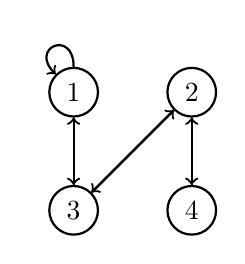
\begin{tikzpicture}[node distance={15mm}, thick, main/.style = {draw, circle}] 
    \node[main] (1) {$1$}; 
    \node[main, right of=1] (2) {$2$};
    \node[main, below of=1] (3) {$3$};
    \node[main, below of=2] (4) {$4$};
    \draw[->] (1) [out=90,in=135,looseness=5] to (1);
    \draw[->] (1) to (3);
    \draw[->] (2) to (3);
    \draw[->] (2) to (4);
    \draw[->] (3) to (1);
    \draw[->] (3) to (2);
    \draw[->] (4) to (2);
\end{tikzpicture} \\

For this problem we calculate the $M^k$ where each element identifies the number of paths of length.
So for example $M^2$ is the number of paths of length 2. \\
$M^2 = M \cdot M$ \\
$M = \begin{bmatrix}
    1 & 0 & 1 & 0 \\
    0 & 0 & 1 & 1 \\
    1 & 1 & 0 & 0 \\
    0 & 1 & 0 & 0 \\
\end{bmatrix}$ \\ 

$M^2 = \begin{bmatrix}
    1 & 0 & 1 & 0 \\
    0 & 0 & 1 & 1 \\
    1 & 1 & 0 & 0 \\
    0 & 1 & 0 & 0 \\
\end{bmatrix} \cdot \begin{bmatrix}
    1 & 0 & 1 & 0 \\
    0 & 0 & 1 & 1 \\
    1 & 1 & 0 & 0 \\
    0 & 1 & 0 & 0 \\
\end{bmatrix}$ \\

$M^2 = \begin{bmatrix}
    1 \cdot 1 + 0 \cdot 0 + 1 \cdot 1 + 0 \cdot 0 & 1 \cdot 0 + 0 \cdot 0 + 1 \cdot 1 + 0 \cdot 1 & 1 \cdot 1 + 0 \cdot 1 + 1 \cdot 0 + 0 \cdot 0 & 1 \cdot 0 + 0 \cdot 1 + 1 \cdot 0 + 0 \cdot 0 \\
    0 \cdot 1 + 0 \cdot 0 + 1 \cdot 1 + 1 \cdot 1 & 0 \cdot 0 + 0 \cdot 0 + 1 \cdot 1 + 1 \cdot 1 & 0 \cdot 1 + 0 \cdot 1 + 1 \cdot 0 + 1 \cdot 0 & 0 \cdot 0 + 0 \cdot 1 + 1 \cdot 0 + 1 \cdot 0 \\
    1 \cdot 1 + 1 \cdot 0 + 0 \cdot 1 + 0 \cdot 0 & 1 \cdot 0 + 1 \cdot 0 + 0 \cdot 1 + 0 \cdot 1 & 1 \cdot 1 + 1 \cdot 1 + 0 \cdot 0 + 0 \cdot 0 & 1 \cdot 0 + 1 \cdot 1 + 0 \cdot 0 + 0 \cdot 0 \\
    0 \cdot 1 + 1 \cdot 0 + 0 \cdot 1 + 0 \cdot 0 & 0 \cdot 0 + 1 \cdot 0 + 0 \cdot 1 + 0 \cdot 1 & 0 \cdot 1 + 1 \cdot 1 + 0 \cdot 0 + 0 \cdot 0 & 0 \cdot 0 + 1 \cdot 1 + 0 \cdot 0 + 0 \cdot 0 \\
\end{bmatrix}$ \\

$M^2 = \begin{bmatrix}
    2 & 1 & 2 & 0 \\
    0 & 0 & 2 & 2 \\
    2 & 2 & 0 & 0 \\
    0 & 2 & 0 & 0 \\
\end{bmatrix}$ \\

Looking at the matrix there must be at least one path of length 2 and length 1\\
Thus this is a transitive relation. \\

Looking at our psuedocode code. \\

\begin{lstlisting}
def transitive(R):
    Rs = R**2
    bOnePass = False
    for i in range(len(Rs)):
        for j in range(len(Rs)):
            if Rs[i][j] == 1:
                bOnePass = True
    if bOnePass:
        bTwoPass = False
        for i in range(len(R)):
            for j in range(len(R)):
                if R[i][j] == 2:
                    bTwoPass = True
                    break
    if bOnePass and bTwoPass:
        return True
    else:
        return False
\end{lstlisting}

\subsubsection{Trichotomy}
In mathematics, the law of trichotomy states that every real number is either positive, negative, or zero.

More generally, a binary relation R on a set X is trichotomous if for all x and y in X, exactly one of xRy, yRx and x=y holds. Writing R as $<$, this is stated in formal logic as: \\

\begin{math}
\forall x \in X \, \forall y \in X \, (
  [       x < y  \, \land \, \lnot(y < x) \, \land \, \lnot(x = y) ] \, \lor \,
  [ \lnot(x < y) \, \land \,       y < x  \, \land \, \lnot(x = y) ] \, \lor \,
  [ \lnot(x < y) \, \land \, \lnot(y < x) \, \land \,       x = y  ]
) \
\end{math} \\
    
A relation is trichotomous if, and only if, it is asymmetric and connected.
If a trichotomous relation is also transitive, then it is a strict total order; this is a special case of a strict weak order.

In a much easier to understand way. \\
For example, the relation $R$ on $A$ is trichotomous. \\

$R = {(1,1),(1,2),(1,3),(2,3)}$ \\ 

$R = \begin{bmatrix}
    1 & 1 & 1 \\
    0 & 0 & 1 \\
    0 & 0 & 0 \\
\end{bmatrix}$ \\

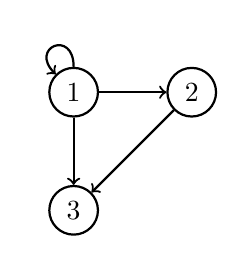
\begin{tikzpicture}[node distance={15mm}, thick, main/.style = {draw, circle}]
    \node[main] (1) {$1$}; 
    \node[main, right of=1] (2) {$2$};
    \node[main, below of=1] (3) {$3$};
    \draw[->] (1) [out=90,in=135,looseness=5] to (1);
    \draw[->] (1) to (2);
    \draw[->] (1) to (3);
    \draw[->] (2) to (3);
\end{tikzpicture} \\

If you notice the relation is trichotomous the relation $R$ is asymmetric and edges are connected only once.

In our psuedocode we can see that we are checking if the relation is trichotomous. \\
\begin{lstlisting}
    def isTrichotomy(self):
        #every pair of nodes has one and only one edge between them.        
        # get all the edges 
        edges = self.R
        # make sure that there are no duplicate edges
        for i in range(len(edges)):
            for j in range(len(edges)):
                if edges[i][0] == edges[j][1] and edges[i][1] == edges[j][0]:
                    return False
        # make sure that there are no edges that are not in the relation                    
        for i in range(len(self.M)):
            for j in range(len(self.M)):
                if self.M[i][j] == 0:
                    for k in range(len(edges)):
                        if edges[k][0] == i+1 and edges[k][1] == j+1:
                            return False
                
        # each node can only have two edges
        for i in range(len(self.M)):
            count = 0
            for j in range(len(self.M)):
                if self.M[i][j] == 1:
                    count += 1
            if count > 2:
                return False
                      
        # must be asymmetric
        if self.isSymmetric():
            return False
            
        return True
\end{lstlisting}



\subsubsection{Equivalence relations}
An \textbf{equivalence} relation is a relation that is \textbf{reflexive}, \textbf{symmetric}, and \textbf{transitive}. \\
An equivalence relation partitions its domain E into disjoint equivalence classes. 
Each equivalence class contains a set of elements of E that are equivalent to each other, and all elements of E equivalent to any element of the equivalence class are members of the equivalence class. 
The equivalence classes are disjoint:  there is no x$\in{E}$ such that x is in more than one equivalence class. 
The equivalence classes exhaust E:  there is no x$\in{E}$ such that x is in no equivalence class. 
Any element of an equivalence class may be its representative; the representative stands for all the members of its equivalence class. 

\subsubsection{Order relations}
An order (or partial order) is a relation that is antisymmetric and transitive. 

A  \textbf{strict} order is one that is \textbf{irreflexive} and  \textbf{transitive}; such an order is also trivially  \textbf{antisymmetric} because there is no x and y such that xRy and yRx. 

A \textbf{non-strict (weak)} order is one that is \textbf{reflexive}, \textbf{antisymmetric}, and \textbf{transitive}. \\

An order relation R on E is a \textbf{total order} if either xRy or yRx $\forall$x,y$\in{E}$. 

An order relation R on E is a \textbf{partial order} if there is a  x,y$\in{E}$ for which neither xRy nor yRx. 

And order relation R on E is a \textbf{Triohotomy} if either xRy, yRx, or x=y $\forall$x,y$\in{E}$.

A \textbf{weak total order} is \textbf{reflexive}, \textbf{antisymmetric}, \textbf{transitive} and \textbf{trichotomy}. \\
A \textbf{strict total order} is \textbf{irreflexive}, \textbf{transitive}, and \textbf{trichotomy}.



\newpage

\end{document}
